% Options for packages loaded elsewhere
\PassOptionsToPackage{unicode}{hyperref}
\PassOptionsToPackage{hyphens}{url}
%
\documentclass[
]{article}
\usepackage{amsmath,amssymb}
\usepackage{lmodern}
\usepackage{iftex}
\ifPDFTeX
  \usepackage[T1]{fontenc}
  \usepackage[utf8]{inputenc}
  \usepackage{textcomp} % provide euro and other symbols
\else % if luatex or xetex
  \usepackage{unicode-math}
  \defaultfontfeatures{Scale=MatchLowercase}
  \defaultfontfeatures[\rmfamily]{Ligatures=TeX,Scale=1}
\fi
% Use upquote if available, for straight quotes in verbatim environments
\IfFileExists{upquote.sty}{\usepackage{upquote}}{}
\IfFileExists{microtype.sty}{% use microtype if available
  \usepackage[]{microtype}
  \UseMicrotypeSet[protrusion]{basicmath} % disable protrusion for tt fonts
}{}
\makeatletter
\@ifundefined{KOMAClassName}{% if non-KOMA class
  \IfFileExists{parskip.sty}{%
    \usepackage{parskip}
  }{% else
    \setlength{\parindent}{0pt}
    \setlength{\parskip}{6pt plus 2pt minus 1pt}}
}{% if KOMA class
  \KOMAoptions{parskip=half}}
\makeatother
\usepackage{xcolor}
\usepackage[margin=1in]{geometry}
\usepackage{color}
\usepackage{fancyvrb}
\newcommand{\VerbBar}{|}
\newcommand{\VERB}{\Verb[commandchars=\\\{\}]}
\DefineVerbatimEnvironment{Highlighting}{Verbatim}{commandchars=\\\{\}}
% Add ',fontsize=\small' for more characters per line
\usepackage{framed}
\definecolor{shadecolor}{RGB}{248,248,248}
\newenvironment{Shaded}{\begin{snugshade}}{\end{snugshade}}
\newcommand{\AlertTok}[1]{\textcolor[rgb]{0.94,0.16,0.16}{#1}}
\newcommand{\AnnotationTok}[1]{\textcolor[rgb]{0.56,0.35,0.01}{\textbf{\textit{#1}}}}
\newcommand{\AttributeTok}[1]{\textcolor[rgb]{0.77,0.63,0.00}{#1}}
\newcommand{\BaseNTok}[1]{\textcolor[rgb]{0.00,0.00,0.81}{#1}}
\newcommand{\BuiltInTok}[1]{#1}
\newcommand{\CharTok}[1]{\textcolor[rgb]{0.31,0.60,0.02}{#1}}
\newcommand{\CommentTok}[1]{\textcolor[rgb]{0.56,0.35,0.01}{\textit{#1}}}
\newcommand{\CommentVarTok}[1]{\textcolor[rgb]{0.56,0.35,0.01}{\textbf{\textit{#1}}}}
\newcommand{\ConstantTok}[1]{\textcolor[rgb]{0.00,0.00,0.00}{#1}}
\newcommand{\ControlFlowTok}[1]{\textcolor[rgb]{0.13,0.29,0.53}{\textbf{#1}}}
\newcommand{\DataTypeTok}[1]{\textcolor[rgb]{0.13,0.29,0.53}{#1}}
\newcommand{\DecValTok}[1]{\textcolor[rgb]{0.00,0.00,0.81}{#1}}
\newcommand{\DocumentationTok}[1]{\textcolor[rgb]{0.56,0.35,0.01}{\textbf{\textit{#1}}}}
\newcommand{\ErrorTok}[1]{\textcolor[rgb]{0.64,0.00,0.00}{\textbf{#1}}}
\newcommand{\ExtensionTok}[1]{#1}
\newcommand{\FloatTok}[1]{\textcolor[rgb]{0.00,0.00,0.81}{#1}}
\newcommand{\FunctionTok}[1]{\textcolor[rgb]{0.00,0.00,0.00}{#1}}
\newcommand{\ImportTok}[1]{#1}
\newcommand{\InformationTok}[1]{\textcolor[rgb]{0.56,0.35,0.01}{\textbf{\textit{#1}}}}
\newcommand{\KeywordTok}[1]{\textcolor[rgb]{0.13,0.29,0.53}{\textbf{#1}}}
\newcommand{\NormalTok}[1]{#1}
\newcommand{\OperatorTok}[1]{\textcolor[rgb]{0.81,0.36,0.00}{\textbf{#1}}}
\newcommand{\OtherTok}[1]{\textcolor[rgb]{0.56,0.35,0.01}{#1}}
\newcommand{\PreprocessorTok}[1]{\textcolor[rgb]{0.56,0.35,0.01}{\textit{#1}}}
\newcommand{\RegionMarkerTok}[1]{#1}
\newcommand{\SpecialCharTok}[1]{\textcolor[rgb]{0.00,0.00,0.00}{#1}}
\newcommand{\SpecialStringTok}[1]{\textcolor[rgb]{0.31,0.60,0.02}{#1}}
\newcommand{\StringTok}[1]{\textcolor[rgb]{0.31,0.60,0.02}{#1}}
\newcommand{\VariableTok}[1]{\textcolor[rgb]{0.00,0.00,0.00}{#1}}
\newcommand{\VerbatimStringTok}[1]{\textcolor[rgb]{0.31,0.60,0.02}{#1}}
\newcommand{\WarningTok}[1]{\textcolor[rgb]{0.56,0.35,0.01}{\textbf{\textit{#1}}}}
\usepackage{graphicx}
\makeatletter
\def\maxwidth{\ifdim\Gin@nat@width>\linewidth\linewidth\else\Gin@nat@width\fi}
\def\maxheight{\ifdim\Gin@nat@height>\textheight\textheight\else\Gin@nat@height\fi}
\makeatother
% Scale images if necessary, so that they will not overflow the page
% margins by default, and it is still possible to overwrite the defaults
% using explicit options in \includegraphics[width, height, ...]{}
\setkeys{Gin}{width=\maxwidth,height=\maxheight,keepaspectratio}
% Set default figure placement to htbp
\makeatletter
\def\fps@figure{htbp}
\makeatother
\setlength{\emergencystretch}{3em} % prevent overfull lines
\providecommand{\tightlist}{%
  \setlength{\itemsep}{0pt}\setlength{\parskip}{0pt}}
\setcounter{secnumdepth}{-\maxdimen} % remove section numbering
\ifLuaTeX
  \usepackage{selnolig}  % disable illegal ligatures
\fi
\IfFileExists{bookmark.sty}{\usepackage{bookmark}}{\usepackage{hyperref}}
\IfFileExists{xurl.sty}{\usepackage{xurl}}{} % add URL line breaks if available
\urlstyle{same} % disable monospaced font for URLs
\hypersetup{
  pdftitle={Bellabeat Case Study - Divyansh Negi},
  hidelinks,
  pdfcreator={LaTeX via pandoc}}

\title{Bellabeat Case Study - Divyansh Negi}
\author{}
\date{2022-08-02}

\begin{document}
\maketitle

\hypertarget{introduction}{%
\subsection{\texorpdfstring{\textbf{\emph{INTRODUCTION}}}{INTRODUCTION}}\label{introduction}}

Welcome to the Bellabeat data analysis case study! In this case study,
we will perform many real-world tasks of a junior data analyst. In order
to answer the key business questions, we will follow the steps of the
data analysis process: \textbf{ask, prepare, process, analyze, share,
and act}.

\hypertarget{scenario}{%
\subsubsection{Scenario}\label{scenario}}

In this study, we will focus on one of Bellabeat's products and analyze
smart device data to gain insight into how consumers are using their
smart devices. The insights we discover will then help guide marketing
strategy for the company. We will be presenting our analysis to the
Bellabeat executive team along with our recommendations for Bellabeat's
marketing strategy.

\hypertarget{about-the-company-bellabeat}{%
\subsubsection{About the Company
Bellabeat}\label{about-the-company-bellabeat}}

Urška Sršen and Sando Mur founded Bellabeat, a high-tech company that
manufactures health-focused smart products. Sršen used her background as
an artist to develop beautifully designed technology that informs and
inspires women around the world. Collecting data on activity, sleep,
stress, and reproductive health has allowed Bellabeat to empower women
with knowledge about their own health and habits. Since it was founded
in 2013, Bellabeat has grown rapidly and quickly positioned itself as a
tech-driven wellness company for women.

\hypertarget{ask-phase}{%
\subsection{\texorpdfstring{\textbf{\emph{ASK
phase}}}{ASK phase}}\label{ask-phase}}

\hypertarget{identifying-the-business-task-}{%
\subsubsection{Identifying the business
task:-}\label{identifying-the-business-task-}}

\begin{itemize}
\tightlist
\item
  \textbf{What are some trends in smart device usage? How could these
  trends help influence Bellabeat marketing strategy ?}
\end{itemize}

The company need to better target their marketing efforts into their
customer's needs based on their usage of their fitness smart devices.
And then, make high-level recommendations for how these trends can
inform Bellabeat marketing strategy.

\begin{itemize}
\tightlist
\item
  \textbf{Who are the main stakeholders ?}
\end{itemize}

The main stakeholders are Urška Sršen, Bellabeat's co-founder and Chief
Creative Officer; Sando Mur, Mathematician and Bellabeat's cofounder;
And also, we need to think about and work with the rest of the Bellabeat
marketing analytics team.

\hypertarget{prepare-phase}{%
\subsection{\texorpdfstring{\textbf{\emph{PREPARE
Phase}}}{PREPARE Phase}}\label{prepare-phase}}

In this phase, we will download and Import the dataset. Then make sure
all the data is organized, credible, sorted and filtered.

\hypertarget{downloading-the-data}{%
\subsubsection{Downloading the data}\label{downloading-the-data}}

We will be using public data that explores smart device users' daily
habits from FitBit Fitness Tracker Data. FitBit Fitness Tracker Data
from Kaggle.

FitBit Fitness Tracker Data :
\url{https://www.kaggle.com/datasets/arashnic/fitbit}

\hypertarget{section}{%
\subsubsection{}\label{section}}

\hypertarget{uploading-the-data}{%
\subsubsection{Uploading the data}\label{uploading-the-data}}

We'll be manually uploading all the data on Rstudio for the analysis in
the working directory.

\hypertarget{loading-the-packages}{%
\subsubsection{Loading the packages}\label{loading-the-packages}}

Now we'll load all the necessary packages that will help us in the
analysis. And in the code we'll be using message=FALSE and
warning=FALSE, to save space. And to prevent printing of the execution
of the R code generated and the warning messages.

\begin{Shaded}
\begin{Highlighting}[]
\CommentTok{\# Installing packages}
\FunctionTok{install.packages}\NormalTok{(}\StringTok{"tidyverse"}\NormalTok{)}
\FunctionTok{install.packages}\NormalTok{(}\StringTok{"lubridate"}\NormalTok{)}
\FunctionTok{install.packages}\NormalTok{(}\StringTok{"dplyr"}\NormalTok{)}
\FunctionTok{install.packages}\NormalTok{(}\StringTok{"ggplot2"}\NormalTok{)}
\FunctionTok{install.packages}\NormalTok{(}\StringTok{"tidyr"}\NormalTok{)}
\end{Highlighting}
\end{Shaded}

Now we'll load the packages.

\begin{Shaded}
\begin{Highlighting}[]
\CommentTok{\# Loading packages }
\FunctionTok{library}\NormalTok{(tidyverse)}
\FunctionTok{library}\NormalTok{(lubridate)}
\FunctionTok{library}\NormalTok{(dplyr)}
\FunctionTok{library}\NormalTok{(ggplot2)}
\FunctionTok{library}\NormalTok{(tidyr)}
\end{Highlighting}
\end{Shaded}

\hypertarget{importing-the-data}{%
\subsubsection{Importing the data}\label{importing-the-data}}

After uploading we'll be importing all dataset. Then we'll VIEW, CLEAN,
FORMAT, and ORGANIZE the data for the analysis.

\begin{itemize}
\tightlist
\item
  \textbf{dailyActivity\_merged.csv}
\end{itemize}

\begin{Shaded}
\begin{Highlighting}[]
\CommentTok{\# Importing Activity dataset :}

\NormalTok{Activity }\OtherTok{\textless{}{-}} \FunctionTok{read.csv}\NormalTok{(}\StringTok{"dailyActivity\_merged.csv"}\NormalTok{)}
\FunctionTok{head}\NormalTok{(Activity)}
\end{Highlighting}
\end{Shaded}

\begin{verbatim}
##           Id ActivityDate TotalSteps TotalDistance TrackerDistance
## 1 1503960366    4/12/2016      13162          8.50            8.50
## 2 1503960366    4/13/2016      10735          6.97            6.97
## 3 1503960366    4/14/2016      10460          6.74            6.74
## 4 1503960366    4/15/2016       9762          6.28            6.28
## 5 1503960366    4/16/2016      12669          8.16            8.16
## 6 1503960366    4/17/2016       9705          6.48            6.48
##   LoggedActivitiesDistance VeryActiveDistance ModeratelyActiveDistance
## 1                        0               1.88                     0.55
## 2                        0               1.57                     0.69
## 3                        0               2.44                     0.40
## 4                        0               2.14                     1.26
## 5                        0               2.71                     0.41
## 6                        0               3.19                     0.78
##   LightActiveDistance SedentaryActiveDistance VeryActiveMinutes
## 1                6.06                       0                25
## 2                4.71                       0                21
## 3                3.91                       0                30
## 4                2.83                       0                29
## 5                5.04                       0                36
## 6                2.51                       0                38
##   FairlyActiveMinutes LightlyActiveMinutes SedentaryMinutes Calories
## 1                  13                  328              728     1985
## 2                  19                  217              776     1797
## 3                  11                  181             1218     1776
## 4                  34                  209              726     1745
## 5                  10                  221              773     1863
## 6                  20                  164              539     1728
\end{verbatim}

\begin{Shaded}
\begin{Highlighting}[]
\FunctionTok{colnames}\NormalTok{(Activity)}
\end{Highlighting}
\end{Shaded}

\begin{verbatim}
##  [1] "Id"                       "ActivityDate"            
##  [3] "TotalSteps"               "TotalDistance"           
##  [5] "TrackerDistance"          "LoggedActivitiesDistance"
##  [7] "VeryActiveDistance"       "ModeratelyActiveDistance"
##  [9] "LightActiveDistance"      "SedentaryActiveDistance" 
## [11] "VeryActiveMinutes"        "FairlyActiveMinutes"     
## [13] "LightlyActiveMinutes"     "SedentaryMinutes"        
## [15] "Calories"
\end{verbatim}

\begin{Shaded}
\begin{Highlighting}[]
\FunctionTok{str}\NormalTok{(Activity)}
\end{Highlighting}
\end{Shaded}

\begin{verbatim}
## 'data.frame':    940 obs. of  15 variables:
##  $ Id                      : num  1.5e+09 1.5e+09 1.5e+09 1.5e+09 1.5e+09 ...
##  $ ActivityDate            : chr  "4/12/2016" "4/13/2016" "4/14/2016" "4/15/2016" ...
##  $ TotalSteps              : int  13162 10735 10460 9762 12669 9705 13019 15506 10544 9819 ...
##  $ TotalDistance           : num  8.5 6.97 6.74 6.28 8.16 ...
##  $ TrackerDistance         : num  8.5 6.97 6.74 6.28 8.16 ...
##  $ LoggedActivitiesDistance: num  0 0 0 0 0 0 0 0 0 0 ...
##  $ VeryActiveDistance      : num  1.88 1.57 2.44 2.14 2.71 ...
##  $ ModeratelyActiveDistance: num  0.55 0.69 0.4 1.26 0.41 ...
##  $ LightActiveDistance     : num  6.06 4.71 3.91 2.83 5.04 ...
##  $ SedentaryActiveDistance : num  0 0 0 0 0 0 0 0 0 0 ...
##  $ VeryActiveMinutes       : int  25 21 30 29 36 38 42 50 28 19 ...
##  $ FairlyActiveMinutes     : int  13 19 11 34 10 20 16 31 12 8 ...
##  $ LightlyActiveMinutes    : int  328 217 181 209 221 164 233 264 205 211 ...
##  $ SedentaryMinutes        : int  728 776 1218 726 773 539 1149 775 818 838 ...
##  $ Calories                : int  1985 1797 1776 1745 1863 1728 1921 2035 1786 1775 ...
\end{verbatim}

\begin{itemize}
\tightlist
\item
  \textbf{dailyCalories\_merged.csv}
\end{itemize}

\begin{Shaded}
\begin{Highlighting}[]
\CommentTok{\# Importing Calories dataset :}
\NormalTok{Calories }\OtherTok{\textless{}{-}} \FunctionTok{read.csv}\NormalTok{(}\StringTok{"dailyCalories\_merged.csv"}\NormalTok{)}
\FunctionTok{head}\NormalTok{(Calories)}
\end{Highlighting}
\end{Shaded}

\begin{verbatim}
##           Id ActivityDay Calories
## 1 1503960366   4/12/2016     1985
## 2 1503960366   4/13/2016     1797
## 3 1503960366   4/14/2016     1776
## 4 1503960366   4/15/2016     1745
## 5 1503960366   4/16/2016     1863
## 6 1503960366   4/17/2016     1728
\end{verbatim}

\begin{Shaded}
\begin{Highlighting}[]
\FunctionTok{colnames}\NormalTok{(Calories)}
\end{Highlighting}
\end{Shaded}

\begin{verbatim}
## [1] "Id"          "ActivityDay" "Calories"
\end{verbatim}

\begin{Shaded}
\begin{Highlighting}[]
\FunctionTok{str}\NormalTok{(Calories)}
\end{Highlighting}
\end{Shaded}

\begin{verbatim}
## 'data.frame':    940 obs. of  3 variables:
##  $ Id         : num  1.5e+09 1.5e+09 1.5e+09 1.5e+09 1.5e+09 ...
##  $ ActivityDay: chr  "4/12/2016" "4/13/2016" "4/14/2016" "4/15/2016" ...
##  $ Calories   : int  1985 1797 1776 1745 1863 1728 1921 2035 1786 1775 ...
\end{verbatim}

\begin{itemize}
\tightlist
\item
  \textbf{dailyIntensities\_merged.csv}
\end{itemize}

\begin{Shaded}
\begin{Highlighting}[]
\CommentTok{\# Importing Intensities dataset :}
\NormalTok{Intensities }\OtherTok{\textless{}{-}} \FunctionTok{read.csv}\NormalTok{(}\StringTok{"dailyIntensities\_merged.csv"}\NormalTok{)}
\FunctionTok{head}\NormalTok{(Intensities)}
\end{Highlighting}
\end{Shaded}

\begin{verbatim}
##           Id ActivityDay SedentaryMinutes LightlyActiveMinutes
## 1 1503960366   4/12/2016              728                  328
## 2 1503960366   4/13/2016              776                  217
## 3 1503960366   4/14/2016             1218                  181
## 4 1503960366   4/15/2016              726                  209
## 5 1503960366   4/16/2016              773                  221
## 6 1503960366   4/17/2016              539                  164
##   FairlyActiveMinutes VeryActiveMinutes SedentaryActiveDistance
## 1                  13                25                       0
## 2                  19                21                       0
## 3                  11                30                       0
## 4                  34                29                       0
## 5                  10                36                       0
## 6                  20                38                       0
##   LightActiveDistance ModeratelyActiveDistance VeryActiveDistance
## 1                6.06                     0.55               1.88
## 2                4.71                     0.69               1.57
## 3                3.91                     0.40               2.44
## 4                2.83                     1.26               2.14
## 5                5.04                     0.41               2.71
## 6                2.51                     0.78               3.19
\end{verbatim}

\begin{Shaded}
\begin{Highlighting}[]
\FunctionTok{colnames}\NormalTok{(Intensities)}
\end{Highlighting}
\end{Shaded}

\begin{verbatim}
##  [1] "Id"                       "ActivityDay"             
##  [3] "SedentaryMinutes"         "LightlyActiveMinutes"    
##  [5] "FairlyActiveMinutes"      "VeryActiveMinutes"       
##  [7] "SedentaryActiveDistance"  "LightActiveDistance"     
##  [9] "ModeratelyActiveDistance" "VeryActiveDistance"
\end{verbatim}

\begin{Shaded}
\begin{Highlighting}[]
\FunctionTok{str}\NormalTok{(Intensities)}
\end{Highlighting}
\end{Shaded}

\begin{verbatim}
## 'data.frame':    940 obs. of  10 variables:
##  $ Id                      : num  1.5e+09 1.5e+09 1.5e+09 1.5e+09 1.5e+09 ...
##  $ ActivityDay             : chr  "4/12/2016" "4/13/2016" "4/14/2016" "4/15/2016" ...
##  $ SedentaryMinutes        : int  728 776 1218 726 773 539 1149 775 818 838 ...
##  $ LightlyActiveMinutes    : int  328 217 181 209 221 164 233 264 205 211 ...
##  $ FairlyActiveMinutes     : int  13 19 11 34 10 20 16 31 12 8 ...
##  $ VeryActiveMinutes       : int  25 21 30 29 36 38 42 50 28 19 ...
##  $ SedentaryActiveDistance : num  0 0 0 0 0 0 0 0 0 0 ...
##  $ LightActiveDistance     : num  6.06 4.71 3.91 2.83 5.04 ...
##  $ ModeratelyActiveDistance: num  0.55 0.69 0.4 1.26 0.41 ...
##  $ VeryActiveDistance      : num  1.88 1.57 2.44 2.14 2.71 ...
\end{verbatim}

\begin{itemize}
\tightlist
\item
  \textbf{heartrate\_seconds\_merged.csv}
\end{itemize}

\begin{Shaded}
\begin{Highlighting}[]
\CommentTok{\# Importing Heartrate dataset :}
\NormalTok{Heartrate }\OtherTok{\textless{}{-}} \FunctionTok{read.csv}\NormalTok{(}\StringTok{"heartrate\_seconds\_merged.csv"}\NormalTok{)}
\FunctionTok{head}\NormalTok{(Heartrate)}
\end{Highlighting}
\end{Shaded}

\begin{verbatim}
##           Id                 Time Value
## 1 2022484408 4/12/2016 7:21:00 AM    97
## 2 2022484408 4/12/2016 7:21:05 AM   102
## 3 2022484408 4/12/2016 7:21:10 AM   105
## 4 2022484408 4/12/2016 7:21:20 AM   103
## 5 2022484408 4/12/2016 7:21:25 AM   101
## 6 2022484408 4/12/2016 7:22:05 AM    95
\end{verbatim}

\begin{Shaded}
\begin{Highlighting}[]
\FunctionTok{colnames}\NormalTok{(Heartrate)}
\end{Highlighting}
\end{Shaded}

\begin{verbatim}
## [1] "Id"    "Time"  "Value"
\end{verbatim}

\begin{Shaded}
\begin{Highlighting}[]
\FunctionTok{str}\NormalTok{(Heartrate)}
\end{Highlighting}
\end{Shaded}

\begin{verbatim}
## 'data.frame':    2483658 obs. of  3 variables:
##  $ Id   : num  2.02e+09 2.02e+09 2.02e+09 2.02e+09 2.02e+09 ...
##  $ Time : chr  "4/12/2016 7:21:00 AM" "4/12/2016 7:21:05 AM" "4/12/2016 7:21:10 AM" "4/12/2016 7:21:20 AM" ...
##  $ Value: int  97 102 105 103 101 95 91 93 94 93 ...
\end{verbatim}

\begin{itemize}
\tightlist
\item
  \textbf{sleepDay\_merged.csv}
\end{itemize}

\begin{Shaded}
\begin{Highlighting}[]
\CommentTok{\# Importing Sleep dataset :}
\NormalTok{Sleep }\OtherTok{\textless{}{-}} \FunctionTok{read.csv}\NormalTok{(}\StringTok{"sleepDay\_merged.csv"}\NormalTok{)}
\FunctionTok{head}\NormalTok{(Sleep)}
\end{Highlighting}
\end{Shaded}

\begin{verbatim}
##           Id              SleepDay TotalSleepRecords TotalMinutesAsleep
## 1 1503960366 4/12/2016 12:00:00 AM                 1                327
## 2 1503960366 4/13/2016 12:00:00 AM                 2                384
## 3 1503960366 4/15/2016 12:00:00 AM                 1                412
## 4 1503960366 4/16/2016 12:00:00 AM                 2                340
## 5 1503960366 4/17/2016 12:00:00 AM                 1                700
## 6 1503960366 4/19/2016 12:00:00 AM                 1                304
##   TotalTimeInBed
## 1            346
## 2            407
## 3            442
## 4            367
## 5            712
## 6            320
\end{verbatim}

\begin{Shaded}
\begin{Highlighting}[]
\FunctionTok{colnames}\NormalTok{(Sleep)}
\end{Highlighting}
\end{Shaded}

\begin{verbatim}
## [1] "Id"                 "SleepDay"           "TotalSleepRecords" 
## [4] "TotalMinutesAsleep" "TotalTimeInBed"
\end{verbatim}

\begin{Shaded}
\begin{Highlighting}[]
\FunctionTok{str}\NormalTok{(Sleep)}
\end{Highlighting}
\end{Shaded}

\begin{verbatim}
## 'data.frame':    413 obs. of  5 variables:
##  $ Id                : num  1.5e+09 1.5e+09 1.5e+09 1.5e+09 1.5e+09 ...
##  $ SleepDay          : chr  "4/12/2016 12:00:00 AM" "4/13/2016 12:00:00 AM" "4/15/2016 12:00:00 AM" "4/16/2016 12:00:00 AM" ...
##  $ TotalSleepRecords : int  1 2 1 2 1 1 1 1 1 1 ...
##  $ TotalMinutesAsleep: int  327 384 412 340 700 304 360 325 361 430 ...
##  $ TotalTimeInBed    : int  346 407 442 367 712 320 377 364 384 449 ...
\end{verbatim}

\begin{itemize}
\tightlist
\item
  \textbf{weightLogInfo\_merged.csv}
\end{itemize}

\begin{Shaded}
\begin{Highlighting}[]
\CommentTok{\# Importing Weight dataset :}
\NormalTok{Weight }\OtherTok{\textless{}{-}} \FunctionTok{read.csv}\NormalTok{(}\StringTok{"weightLogInfo\_merged.csv"}\NormalTok{)}
\FunctionTok{head}\NormalTok{(Weight)}
\end{Highlighting}
\end{Shaded}

\begin{verbatim}
##           Id                  Date WeightKg WeightPounds Fat   BMI
## 1 1503960366  5/2/2016 11:59:59 PM     52.6     115.9631  22 22.65
## 2 1503960366  5/3/2016 11:59:59 PM     52.6     115.9631  NA 22.65
## 3 1927972279  4/13/2016 1:08:52 AM    133.5     294.3171  NA 47.54
## 4 2873212765 4/21/2016 11:59:59 PM     56.7     125.0021  NA 21.45
## 5 2873212765 5/12/2016 11:59:59 PM     57.3     126.3249  NA 21.69
## 6 4319703577 4/17/2016 11:59:59 PM     72.4     159.6147  25 27.45
##   IsManualReport        LogId
## 1           True 1.462234e+12
## 2           True 1.462320e+12
## 3          False 1.460510e+12
## 4           True 1.461283e+12
## 5           True 1.463098e+12
## 6           True 1.460938e+12
\end{verbatim}

\begin{Shaded}
\begin{Highlighting}[]
\FunctionTok{colnames}\NormalTok{(Weight)}
\end{Highlighting}
\end{Shaded}

\begin{verbatim}
## [1] "Id"             "Date"           "WeightKg"       "WeightPounds"  
## [5] "Fat"            "BMI"            "IsManualReport" "LogId"
\end{verbatim}

\begin{Shaded}
\begin{Highlighting}[]
\FunctionTok{str}\NormalTok{(Weight)}
\end{Highlighting}
\end{Shaded}

\begin{verbatim}
## 'data.frame':    67 obs. of  8 variables:
##  $ Id            : num  1.50e+09 1.50e+09 1.93e+09 2.87e+09 2.87e+09 ...
##  $ Date          : chr  "5/2/2016 11:59:59 PM" "5/3/2016 11:59:59 PM" "4/13/2016 1:08:52 AM" "4/21/2016 11:59:59 PM" ...
##  $ WeightKg      : num  52.6 52.6 133.5 56.7 57.3 ...
##  $ WeightPounds  : num  116 116 294 125 126 ...
##  $ Fat           : int  22 NA NA NA NA 25 NA NA NA NA ...
##  $ BMI           : num  22.6 22.6 47.5 21.5 21.7 ...
##  $ IsManualReport: chr  "True" "True" "False" "True" ...
##  $ LogId         : num  1.46e+12 1.46e+12 1.46e+12 1.46e+12 1.46e+12 ...
\end{verbatim}

All datasets have been improrted.

\hypertarget{process-phase}{%
\subsection{\texorpdfstring{\textbf{\emph{Process
Phase}}}{Process Phase}}\label{process-phase}}

\hypertarget{cleaning}{%
\subsubsection{Cleaning}\label{cleaning}}

Now, we'll Process, Clean and Organize the dataset for analysis.

We'll install and load the packages for cleaning:

\begin{Shaded}
\begin{Highlighting}[]
\CommentTok{\# Installing package}
\FunctionTok{install.packages}\NormalTok{(}\StringTok{"tidyverse"}\NormalTok{)}
\FunctionTok{library}\NormalTok{(janitor)}
\end{Highlighting}
\end{Shaded}

We'll clean the names of the data using clean\_names().

\begin{Shaded}
\begin{Highlighting}[]
\FunctionTok{clean\_names}\NormalTok{(Activity)}
\FunctionTok{clean\_names}\NormalTok{(Calories)}
\FunctionTok{clean\_names}\NormalTok{(Weight)}
\FunctionTok{clean\_names}\NormalTok{(Heartrate)}
\FunctionTok{clean\_names}\NormalTok{(Intensities)}
\FunctionTok{clean\_names}\NormalTok{(Sleep)}
\end{Highlighting}
\end{Shaded}

And some other cleaning steps we performed with the data :

\begin{itemize}
\item
  For Dataset (Activity, Calories and Intensities): No Spelling errors,
  Misfiled values, Missing values, Extra and blank space, no duplicated
  were found.
\item
  For Sleep data : 3 duplicates were found and removed.
\item
  For Weight data : too many missing values were found in one column. So
  we removed that column.
\end{itemize}

\hypertarget{analyse-phase}{%
\subsection{\texorpdfstring{\textbf{\emph{ANALYSE
Phase}}}{ANALYSE Phase}}\label{analyse-phase}}

After storing all the data and preparing it for analysis. We can start
the analysis.

Let's look at the total number of participants in each data sets:

\begin{Shaded}
\begin{Highlighting}[]
\FunctionTok{n\_distinct}\NormalTok{(Activity}\SpecialCharTok{$}\NormalTok{Id)}
\end{Highlighting}
\end{Shaded}

\begin{verbatim}
## [1] 33
\end{verbatim}

\begin{Shaded}
\begin{Highlighting}[]
\FunctionTok{n\_distinct}\NormalTok{(Calories}\SpecialCharTok{$}\NormalTok{Id)}
\end{Highlighting}
\end{Shaded}

\begin{verbatim}
## [1] 33
\end{verbatim}

\begin{Shaded}
\begin{Highlighting}[]
\FunctionTok{n\_distinct}\NormalTok{(Intensities}\SpecialCharTok{$}\NormalTok{Id)}
\end{Highlighting}
\end{Shaded}

\begin{verbatim}
## [1] 33
\end{verbatim}

\begin{Shaded}
\begin{Highlighting}[]
\FunctionTok{n\_distinct}\NormalTok{(Heartrate}\SpecialCharTok{$}\NormalTok{Id)}
\end{Highlighting}
\end{Shaded}

\begin{verbatim}
## [1] 14
\end{verbatim}

\begin{Shaded}
\begin{Highlighting}[]
\FunctionTok{n\_distinct}\NormalTok{(Sleep}\SpecialCharTok{$}\NormalTok{Id)}
\end{Highlighting}
\end{Shaded}

\begin{verbatim}
## [1] 24
\end{verbatim}

\begin{Shaded}
\begin{Highlighting}[]
\FunctionTok{n\_distinct}\NormalTok{(Weight}\SpecialCharTok{$}\NormalTok{Id)}
\end{Highlighting}
\end{Shaded}

\begin{verbatim}
## [1] 8
\end{verbatim}

So, there are 33 participants in the activity, calories and intensities
data sets. 24 participants in the Sleep data. And only 14 participants
for Heartrate, and only 8 in the weight data set. 8 and 14 participants
are not significant to make any recommendations and conclusions based on
these dataset.

So I will focus on these datasets for my analysis: Activity, Calories,
Intensities and Sleep.

Here are some quick summary statistics about each data frame.

For the Activity dataframe:

\begin{Shaded}
\begin{Highlighting}[]
\CommentTok{\# Activity}
\NormalTok{Activity }\SpecialCharTok{\%\textgreater{}\%}  
  \FunctionTok{select}\NormalTok{(TotalSteps,}
\NormalTok{         TotalDistance,}
\NormalTok{         SedentaryMinutes, Calories) }\SpecialCharTok{\%\textgreater{}\%}
  \FunctionTok{summary}\NormalTok{()}
\end{Highlighting}
\end{Shaded}

\begin{verbatim}
##    TotalSteps    TotalDistance    SedentaryMinutes    Calories   
##  Min.   :    0   Min.   : 0.000   Min.   :   0.0   Min.   :   0  
##  1st Qu.: 3790   1st Qu.: 2.620   1st Qu.: 729.8   1st Qu.:1828  
##  Median : 7406   Median : 5.245   Median :1057.5   Median :2134  
##  Mean   : 7638   Mean   : 5.490   Mean   : 991.2   Mean   :2304  
##  3rd Qu.:10727   3rd Qu.: 7.713   3rd Qu.:1229.5   3rd Qu.:2793  
##  Max.   :36019   Max.   :28.030   Max.   :1440.0   Max.   :4900
\end{verbatim}

Exploring the number of Intense active participants :

\begin{Shaded}
\begin{Highlighting}[]
\CommentTok{\# Explore number of active minutes per category}
\NormalTok{Intensities }\SpecialCharTok{\%\textgreater{}\%}
  \FunctionTok{select}\NormalTok{(VeryActiveMinutes, FairlyActiveMinutes, LightlyActiveMinutes, SedentaryMinutes) }\SpecialCharTok{\%\textgreater{}\%}
  \FunctionTok{summary}\NormalTok{()}
\end{Highlighting}
\end{Shaded}

\begin{verbatim}
##  VeryActiveMinutes FairlyActiveMinutes LightlyActiveMinutes SedentaryMinutes
##  Min.   :  0.00    Min.   :  0.00      Min.   :  0.0        Min.   :   0.0  
##  1st Qu.:  0.00    1st Qu.:  0.00      1st Qu.:127.0        1st Qu.: 729.8  
##  Median :  4.00    Median :  6.00      Median :199.0        Median :1057.5  
##  Mean   : 21.16    Mean   : 13.56      Mean   :192.8        Mean   : 991.2  
##  3rd Qu.: 32.00    3rd Qu.: 19.00      3rd Qu.:264.0        3rd Qu.:1229.5  
##  Max.   :210.00    Max.   :143.00      Max.   :518.0        Max.   :1440.0
\end{verbatim}

For the Calories dataframe:

\begin{Shaded}
\begin{Highlighting}[]
\CommentTok{\# Calories}
\NormalTok{Calories }\SpecialCharTok{\%\textgreater{}\%}
  \FunctionTok{select}\NormalTok{(Calories) }\SpecialCharTok{\%\textgreater{}\%}
  \FunctionTok{summary}\NormalTok{()}
\end{Highlighting}
\end{Shaded}

\begin{verbatim}
##     Calories   
##  Min.   :   0  
##  1st Qu.:1828  
##  Median :2134  
##  Mean   :2304  
##  3rd Qu.:2793  
##  Max.   :4900
\end{verbatim}

For the Sleep dataframe:

\begin{Shaded}
\begin{Highlighting}[]
\CommentTok{\# Sleep}
\NormalTok{Sleep }\SpecialCharTok{\%\textgreater{}\%}
  \FunctionTok{select}\NormalTok{(TotalSleepRecords, TotalMinutesAsleep, TotalTimeInBed) }\SpecialCharTok{\%\textgreater{}\%}
  \FunctionTok{summary}\NormalTok{()}
\end{Highlighting}
\end{Shaded}

\begin{verbatim}
##  TotalSleepRecords TotalMinutesAsleep TotalTimeInBed 
##  Min.   :1.000     Min.   : 58.0      Min.   : 61.0  
##  1st Qu.:1.000     1st Qu.:361.0      1st Qu.:403.0  
##  Median :1.000     Median :433.0      Median :463.0  
##  Mean   :1.119     Mean   :419.5      Mean   :458.6  
##  3rd Qu.:1.000     3rd Qu.:490.0      3rd Qu.:526.0  
##  Max.   :3.000     Max.   :796.0      Max.   :961.0
\end{verbatim}

For the Weight dataframe:

\begin{Shaded}
\begin{Highlighting}[]
\CommentTok{\# Weight}
\NormalTok{Weight }\SpecialCharTok{\%\textgreater{}\%}
  \FunctionTok{select}\NormalTok{(WeightKg, Fat) }\SpecialCharTok{\%\textgreater{}\%}
  \FunctionTok{summary}\NormalTok{()}
\end{Highlighting}
\end{Shaded}

\begin{verbatim}
##     WeightKg           Fat       
##  Min.   : 52.60   Min.   :22.00  
##  1st Qu.: 61.40   1st Qu.:22.75  
##  Median : 62.50   Median :23.50  
##  Mean   : 72.04   Mean   :23.50  
##  3rd Qu.: 85.05   3rd Qu.:24.25  
##  Max.   :133.50   Max.   :25.00  
##                   NA's   :65
\end{verbatim}

\hypertarget{findings}{%
\subsubsection{Findings:}\label{findings}}

\begin{itemize}
\tightlist
\item
  The average sedentary time is too high (more than 16 hours). Which can
  be reduced with a good marketing strategy.
\item
  The majority of the participants are lightly active. With a high
  sedentary time.
\item
  Participants sleep 1 time for an average of 7 hours.
\item
  Average total steps per day (which is 7638) is a little bit less than
  recommended by the CDC. According to the CDC research, taking 8,000
  steps per day was associated with a 51\% lower risk for all-cause
  mortality (or death from all causes). And taking 12,000 steps per day
  was associated with a 65\% lower risk compared with taking 4,000
  steps.
\end{itemize}

\hypertarget{share-and-act-phases}{%
\subsection{\texorpdfstring{\textbf{\emph{SHARE and ACT
Phases}}}{SHARE and ACT Phases}}\label{share-and-act-phases}}

Now we'll visualize some findings.

\hypertarget{relationship-between-steps-and-sedentary-time}{%
\subsubsection{\texorpdfstring{* \textbf{Relationship between Steps and
Sedentary
time}}{* Relationship between Steps and Sedentary time}}\label{relationship-between-steps-and-sedentary-time}}

\begin{Shaded}
\begin{Highlighting}[]
\FunctionTok{ggplot}\NormalTok{(}\AttributeTok{data=}\NormalTok{Activity, }\FunctionTok{aes}\NormalTok{(}\AttributeTok{x=}\NormalTok{TotalSteps, }\AttributeTok{y=}\NormalTok{SedentaryMinutes)) }\SpecialCharTok{+} \FunctionTok{geom\_point}\NormalTok{() }\SpecialCharTok{+} \FunctionTok{geom\_smooth}\NormalTok{() }\SpecialCharTok{+} \FunctionTok{labs}\NormalTok{(}\AttributeTok{title=}\StringTok{"Total Steps vs. Sedentary Minutes"}\NormalTok{)}
\end{Highlighting}
\end{Shaded}

\begin{verbatim}
## `geom_smooth()` using method = 'loess' and formula 'y ~ x'
\end{verbatim}

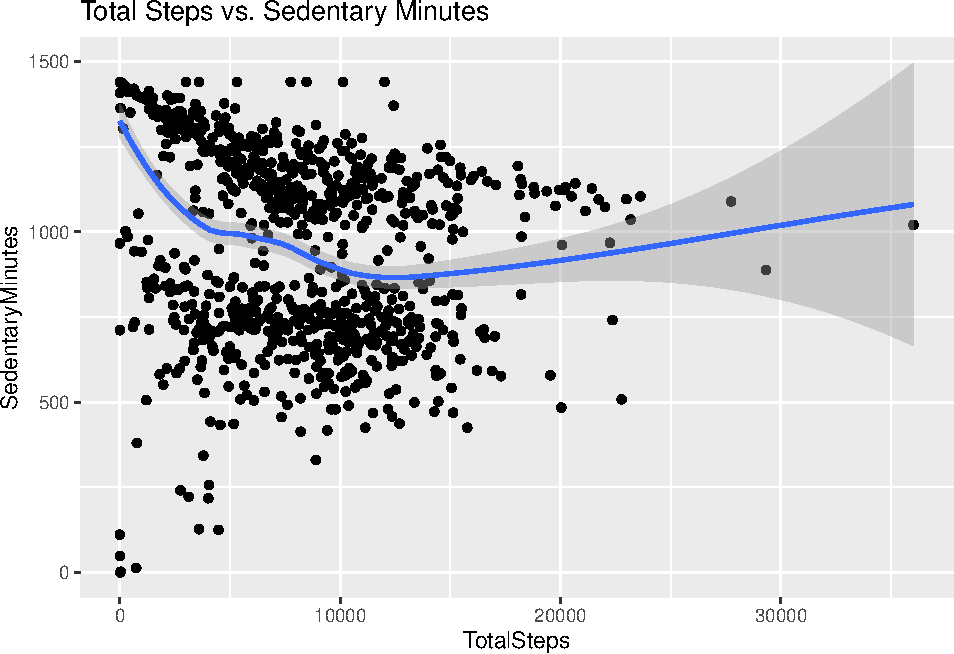
\includegraphics{Bellabeat_files/figure-latex/unnamed-chunk-17-1.pdf} We
can see a negative correlation between Steps and Sedentary time. The
more Sedentary time you have, the less Steps you're taking during the
day. This data shows that the company need to market more the customer
segments with high Sedentary time. And to do that, the company needs to
find ways to get customers get started in walking more and also measure
their daily steps.

\hypertarget{relationship-between-minutes-asleep-and-time-in-bed}{%
\subsubsection{\texorpdfstring{* \textbf{Relationship between Minutes
Asleep and Time in
Bed}}{* Relationship between Minutes Asleep and Time in Bed}}\label{relationship-between-minutes-asleep-and-time-in-bed}}

\begin{Shaded}
\begin{Highlighting}[]
\FunctionTok{ggplot}\NormalTok{(}\AttributeTok{data=}\NormalTok{Sleep, }\FunctionTok{aes}\NormalTok{(}\AttributeTok{x=}\NormalTok{TotalMinutesAsleep, }\AttributeTok{y=}\NormalTok{TotalTimeInBed)) }\SpecialCharTok{+} \FunctionTok{geom\_line}\NormalTok{() }\SpecialCharTok{+}\FunctionTok{geom\_smooth}\NormalTok{() }\SpecialCharTok{+} \FunctionTok{labs}\NormalTok{(}\AttributeTok{title =}\StringTok{"Total Minutes Asleep vs. Total Time In Bed"}\NormalTok{)}
\end{Highlighting}
\end{Shaded}

\begin{verbatim}
## `geom_smooth()` using method = 'loess' and formula 'y ~ x'
\end{verbatim}

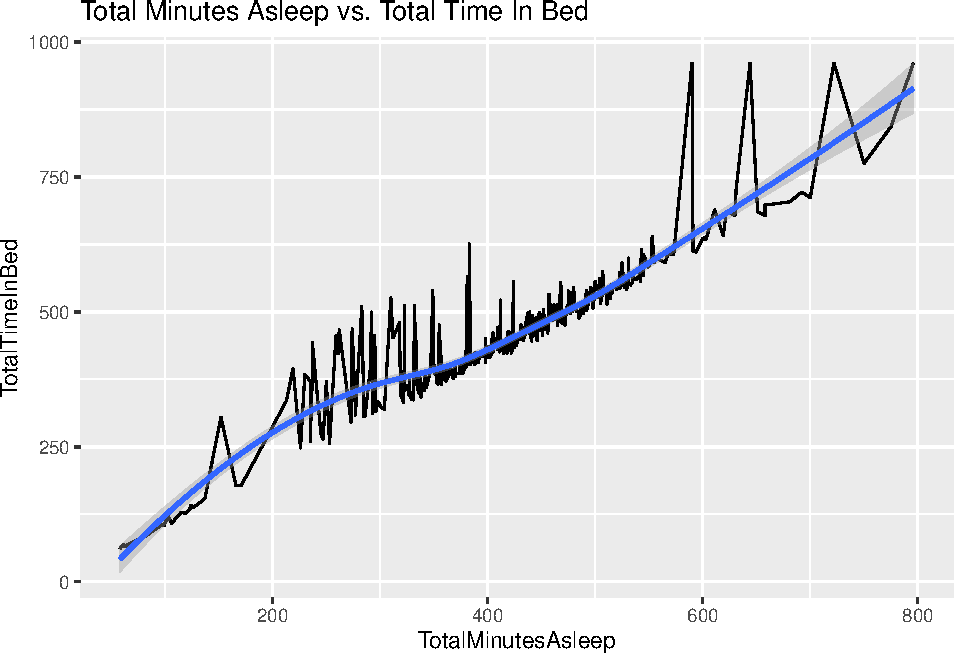
\includegraphics{Bellabeat_files/figure-latex/unnamed-chunk-18-1.pdf} We
can see here an almost completely linear trend between Minutes Asleep
and Time in Bed. So to help users improve their sleep, the company
should consider using notification to go to sleep.

\hypertarget{relationship-between-steps-and-calories}{%
\subsubsection{\texorpdfstring{* \textbf{Relationship between Steps and
Calories}}{* Relationship between Steps and Calories}}\label{relationship-between-steps-and-calories}}

\begin{Shaded}
\begin{Highlighting}[]
\FunctionTok{ggplot}\NormalTok{(}\AttributeTok{data=}\NormalTok{Activity, }\FunctionTok{aes}\NormalTok{(}\AttributeTok{x=}\NormalTok{TotalSteps, }\AttributeTok{y=}\NormalTok{Calories)) }\SpecialCharTok{+} \FunctionTok{geom\_point}\NormalTok{() }\SpecialCharTok{+} \FunctionTok{geom\_smooth}\NormalTok{() }\SpecialCharTok{+} \FunctionTok{labs}\NormalTok{(}\AttributeTok{title=}\StringTok{"Total Steps vs. Calories"}\NormalTok{)}
\end{Highlighting}
\end{Shaded}

\begin{verbatim}
## `geom_smooth()` using method = 'loess' and formula 'y ~ x'
\end{verbatim}

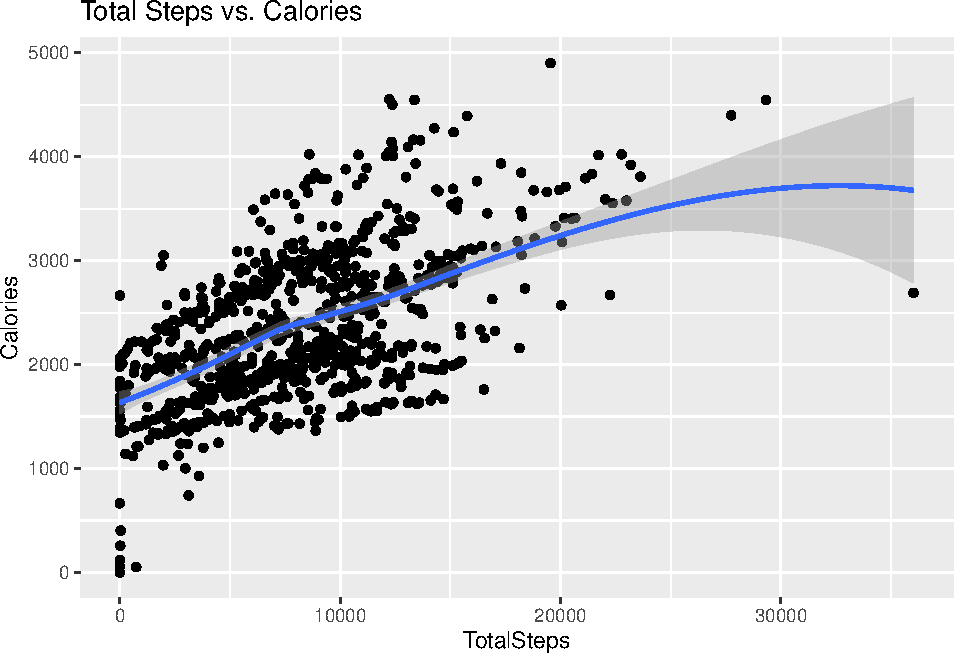
\includegraphics{Bellabeat_files/figure-latex/unnamed-chunk-19-1.pdf} We
can see here a positive correlation between Total Steps and Calories.
The more active we are, the more calories we will burn.

\hypertarget{conclusions-recommandations}{%
\subsection{\texorpdfstring{\textbf{\emph{Conclusions \&
Recommandations}}}{Conclusions \& Recommandations}}\label{conclusions-recommandations}}

So, collecting data on activity, sleep, stress, etc. will allow the
company Bellabeat to empower the customers with knowledge about their
own health and daily habits. The company Bellabeat is growing rapidly
and quickly positioned itself as a tech-driven wellness company for
their customers.

By analyzing the FitBit Fitness Tracker Data set, We have found some
insights that would help influence Bellabeat marketing strategy.

\begin{itemize}
\item
  The average sedentary time is too high for the users of the app (more
  than 16 hours). And definitely needs to be reduced with a good
  marketing strategy. So, the data shows that the company need to market
  more to the customer segment with a high Sedentary time. And to do
  that, the company needs to find ways to get customers started in
  walking more by measuring their daily steps (+ notifications).
\item
  Participants sleep 1 time for an average of 7 hours. To help users
  improve their sleep, Bellabeat should consider using app notifications
  to go to bed.
\item
  The average total steps per day (which is 7638) is a little bit less
  than recommended by the CDC. According to the CDC research, taking
  8,000 steps per day was associated with a 51\% lower risk for
  all-cause mortality (or death from all causes). And taking 12,000
  steps per day was associated with a 65\% lower risk compared with
  taking 4,000 steps. So, Bellabeat can encourage people to take at
  least 8,000 steps per day by explaining the healthy benefits of doing
  that.
\item
  For customers who want to lose weight, it can be a good idea to
  control daily calorie consumption. And Bellabeat can suggest some
  ideas for low-calorie healthy food.
\end{itemize}

\textbf{Hence, the case study has been concluded.}

\end{document}
